% =====================================================================
% Fig.6 -- Prototype usage entropy per TAB block, balance loss on vs off.
% outline.md §3.6 (routing interpretability) / traceability C4 ("usage 分布").
% Self-contained pgfplots figure; \input into the paper.
% Requires in preamble: \usepackage{pgfplots}\pgfplotsset{compat=1.16}
% DATA PROVENANCE (verbatim, no fabrication):
%   paper/plan/ablation-results-to-fill.md Section 5c (per-block usage entropy),
%   x4 ablation on Urban100, representative seed 3407. Per-block
%   prototype count M = [16,32,64,128,16,32,64,128] (catanet_arch.py:516). Higher
%   entropy = more balanced prototype usage. "balance on" = full model; "balance
%   off" = route_balance_weight all 0 (A3_balance_off).
% Block means: on 0.686 vs off 0.623 (raised in ALL 8 blocks).
% =====================================================================
\begin{figure}[H]
\centering
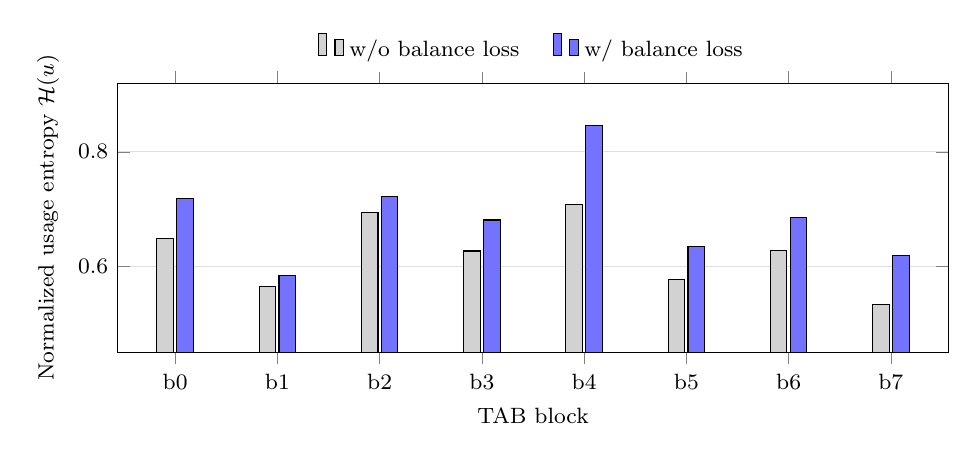
\begin{tikzpicture}
\begin{axis}[
    width=\linewidth, height=5.0cm,
    ybar=1.2pt, bar width=6pt,
    enlarge x limits=0.08,
    ymin=0.45, ymax=0.92,
    ymajorgrids, grid style={gray!25},
    ylabel={Normalized usage entropy $\mathcal{H}(u)$},
    xlabel={TAB block},
    symbolic x coords={b0,b1,b2,b3,b4,b5,b6,b7},
    xtick=data,
    tick label style={font=\footnotesize},
    label style={font=\footnotesize},
    legend style={font=\footnotesize, at={(0.5,1.04)}, anchor=south,
                  legend columns=2, draw=none, /tikz/every even column/.append style={column sep=10pt}},
]
% balance off (route_balance_weight = 0)
\addplot+[draw=black, fill=gray!35] coordinates {
  (b0,0.6482) (b1,0.5655) (b2,0.6947) (b3,0.6268)
  (b4,0.7088) (b5,0.5764) (b6,0.6279) (b7,0.5332) };
% balance on (full model, default weights)
\addplot+[draw=black, fill=blue!55] coordinates {
  (b0,0.7181) (b1,0.5845) (b2,0.7227) (b3,0.6810)
  (b4,0.8466) (b5,0.6352) (b6,0.6848) (b7,0.6193) };
\legend{w/o balance loss, w/ balance loss}
\end{axis}
\end{tikzpicture}
\caption{Normalized prototype-usage entropy $\mathcal{H}(u)$ (Eq.~\eqref{eq:balance};
higher $=$ more balanced) per TAB block ($b_0$--$b_7$) at $\times4$ on Urban100 (full
model, representative seed $3407$). The usage-balancing regularizer increases the entropy in
\emph{all eight} blocks (block-mean $0.623\!\rightarrow\!0.686$), confirming that it counteracts
the collapse onto a few prototypes encouraged by the learnable temperature (C4).}
\label{fig:usage_entropy}
\end{figure}
